\documentclass[UFT8]{beamer}
\usepackage{tikz}
\usetikzlibrary{arrows, positioning, shapes.geometric, arrows.meta}

\mode<presentation> {
	\usetheme{Frankfurt}
	% or AnnArbor Antibes Bergen Berkeley Berlin Boadilla boxes CambridgeUS Copenhagen Darmstadt default Dresden Frankfurt Goettingen Hannover Ilmenau JuanLesPinsLuebeck Madrid Malmoe Marburg Montpellier PaloAlto Pittsburgh Rochester Singapore Szeged Warsaw
	
	\setbeamercovered{transparent}
	% or whatever (possibly just delete it)
}

\usepackage{color}
\usepackage{algorithm,algpseudocode}
\usepackage{algorithmicx}
\usepackage{algpseudocode}
\usepackage{amsmath}
\usepackage{float}

\usefonttheme[onlymath]{serif}

% \documentclass[ppt.tex]{subfiles}
\begin{document}

\section{{Commitment}}

\begin{frame}
    \frametitle{Hiding and Binding}
	\begin{definition}[Hiding commitment]
		A commitment scheme is said to be hiding if for all PPT adversaries $\mathcal{A}$
		\begin{equation*}
			\left\lvert \Pr\left[
				\begin{aligned}
					pp \leftarrow Setup; (x_0, x_1) \leftarrow \mathcal{A}; \\
					b \leftarrow_R \{0, 1\}, r \leftarrow_R \{0, 1\} \\
					\mathcal{C} = Com(x_b; {\color{red}r});
					b' \leftarrow \mathcal{A}(pp, \mathcal{C}) 
				\end{aligned}: b = b'
			\right] - \frac{1}{2} \right\rvert \le \epsilon(\kappa)
		\end{equation*}
	\end{definition}

	\begin{definition}[Binding commitment]
		A commitment scheme is binding if for all PPT adversaries $\mathcal{A}$
		\begin{equation*}
			\Pr\left[
				\begin{aligned}
					pp \leftarrow Setup;\\
					(x_0, x_1, r_0, r_1) \leftarrow \mathcal{A};
				\end{aligned}: \begin{aligned}
					Com(x_0; r_0) = Com(x_1; r_1) \\
					\land x_0 \neq x_1
				\end{aligned}
			\right] \le \epsilon(\kappa)
		\end{equation*}
	\end{definition}
\end{frame}

\begin{frame}
	\frametitle{Controversial Definitions of Polynomial Commitment}
	\begin{figure}
		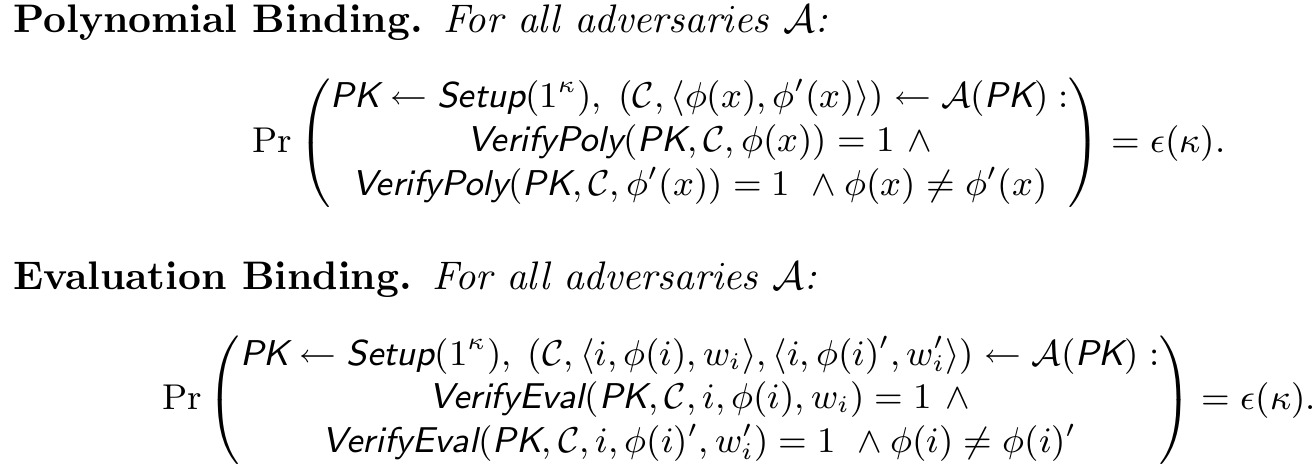
\includegraphics[scale=0.35]{assets/kzg-pcs.png}
	\end{figure}
	\begin{itemize}
		\item No relation between evaluation and polynomial 
	\end{itemize}
	\begin{figure}
		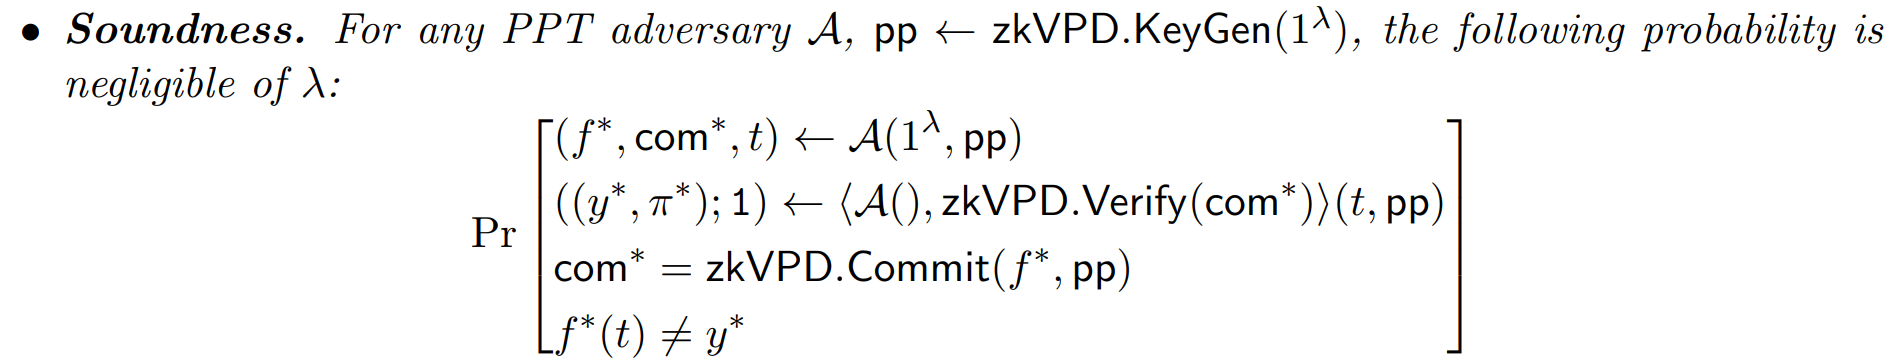
\includegraphics[scale=0.32]{assets/virgo-pcs.png}
	\end{figure}
	\begin{itemize}
		\item Object of interative proof is ambiguous
	\end{itemize}
\end{frame}

\begin{frame}
	\frametitle{Polynomial Commitment}

	\begin{definition}[Polynomial commitment scheme, from Brakedown]
	\begin{itemize}
		\item $pp \leftarrow Setup(1^{\lambda}, t)$: $t$ is degree
		\item $(\mathcal{C}, d) \leftarrow Commit(pp, \mathcal{F})$, input polynomial $\mathcal{F}$, output commitment and decommitment information $d$
		\item $b \leftarrow Open(pp, \mathcal{C}, d, \mathcal{F})$, verifies the opening of commitment, output $b \in \{0, 1\}$
		\item $b \leftarrow Eval(pp, \mathcal{C}, z, y, t, \mathcal{F})$ is a protocol between a PPT prover $\mathcal{P}$ and verifier $\mathcal{V}$. $z$ is the evaluation point, $y$ is evaluation. $b = \langle \mathcal{P}(\mathcal{F}), \mathcal{V} \rangle(pp, \mathcal{C}, z, y, t) \in \{0, 1\}$.
	\end{itemize}
	\end{definition}
\end{frame}

\begin{frame}
	\frametitle{Polynomial Commitment}

	\begin{definition}[Polynomial commitment scheme, from Brakedown]
	\begin{itemize}
		\item Binding. For any PPT adversary $\mathcal{A}$,
		\begin{equation*}
			\Pr\left[
				\begin{aligned}
					pp \leftarrow Setup;  \\
					(\mathcal{C}, d_1, \mathcal{F}_1, d_2, \mathcal{F}_2) \leftarrow \mathcal{A}(pp); \\
					b_0 \leftarrow Open(pp, \mathcal{C}, d_1, \mathcal{F}_1); \\
					b_1 \leftarrow Open(pp, \mathcal{C}, d_2, \mathcal{F}_2);
				\end{aligned} : \begin{aligned}
					b_0 = 1 \land b_1 = 1 \\
					\land \mathcal{F}_1 \neq \mathcal{F}_2
				\end{aligned}
			\right]
		\end{equation*}
		\item (Knowledge) Soundness: $Eval$ is an argument (of knowledge) for the following NP relation given $pp$
		\begin{equation*}
			\left\{\langle 
				(\mathcal{C}, z, y), (\mathcal{F}, d) 
			\rangle: \begin{aligned}
				\mathcal{F} \in \mathbb{F}[t] \land \mathcal{F}(z) = y \land \\
				Open(pp, \mathcal{C}, \mathcal{F}, d) = 1
			\end{aligned}
			\right\}
		\end{equation*}
	\end{itemize}
	\end{definition}
\end{frame}

\begin{frame}
	\frametitle{Difficulty in defining zero knowledge property}
	Strawman: $Eval$ is a zero knowledge interactive proof.

	Two bugs:
	\begin{itemize}
		\item Let $\mathcal{C} = \mathcal{F}$. The scheme leaks the whole polynomial, but it's "zero knowledge" (can be fixed by adding Hiding property) 
		\item For hash-based polynomial commitment, $\mathcal{C}$ is a hash root.
		The interactive protocol must open the hash result, while the simulator can't.
		So all hash-based polynomial commitment can't be zero-knowledge.
	\end{itemize}
\end{frame}


\begin{frame}
    \frametitle{Honest Verifier Zero Knowledge (From Virgo)}
	There is simulator $\mathcal{S}_1, \mathcal{S}_2$ for all polynomial $f$, PPT non-uniform adversary $\mathcal{A}$:
	\begin{align*}
		\Pr\left[\begin{aligned}
			\mathcal{C} \leftarrow Commit(pp, f) \\
			z \leftarrow \mathcal{A}(\mathcal{C}, pp) \\
			(y, tr) \leftarrow \langle 
				\mathcal{P}(f), \mathcal{V}
			\rangle(z) \\
			b \leftarrow \mathcal{A}(\mathcal{C}, y, z, tr)
		\end{aligned}:
		b = 1
		\right] = 
		\Pr\left[\begin{aligned}
			\mathcal{C} \leftarrow \mathcal{S}_1(pp) \\
			z \leftarrow \mathcal{A}(\mathcal{C}, pp) \\
			(y, tr) \leftarrow \mathcal{S}_2(z) \\
			{\color{red}\text{given oracle } f(z)} \\
			b \leftarrow \mathcal{A}(\mathcal{C}, y, z, tr)
		\end{aligned}:
		b = 1
		\right]
	\end{align*}
	\begin{itemize}
		\item $z$ is chosen by $\mathcal{A}$
		\item Satisfying hiding and zero knowledge evaluation property
		\item $\mathcal{S}_2$ needs oracle access to $f(z)$
	\end{itemize}
\end{frame}

\end{document}